\chapter{Images, Toasts and Sound}

\section{Introduction}
...To be filled...

\section{Supporting Different Screens}
\label{lec7:supportDiffScreens}
Due to the growing popularity of android OS each year new vendors enter the market introducing new android smart phones. This resulted in a lot of devices being completely different from each other, different screen sizes, different OS versions, different pixel densities etc. This phenomena is known as ``device fragmentation''. One aspect, the screen size fragmentation is depicted in the figure below:

\begin{center}
	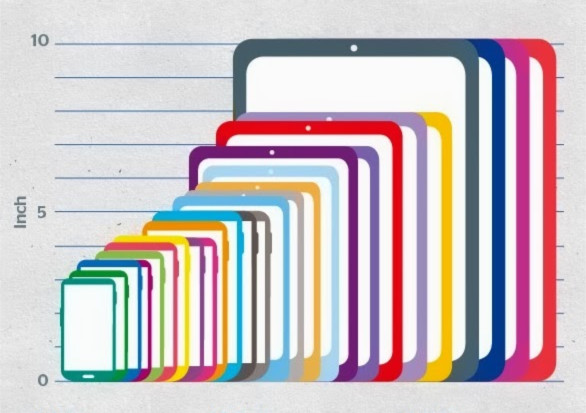
\includegraphics[scale=0.4]{chapters/ch06/images/1}
\end{center} 

To give you an idea of the diversity of the devices, there are currently 1300 unique brands operating in the mobile market! You can check out the complete fragmentation statistics report for the year 2015 \href{http://opensignal.com/reports/2015/08/android-fragmentation/}{at this link}. 

\subsection{Device Independent Pixels}
\label{lec07:dp}
Even if two mobile devices have the same physical screen sizes, they can have dramatically different resolutions. Both of the following devices have physical screen size of 4 inches. For the sake of example let's suppose that device \texttt{A} (left side) has a resolution of 4 pixels by 6 pixels. The device \texttt{B} (right side) is a different device having same physical screen size but a resolution \textbf{4 times} higher i.e: 16 pixels by 24 pixels. Each black square is a pixel:

\begin{center}
	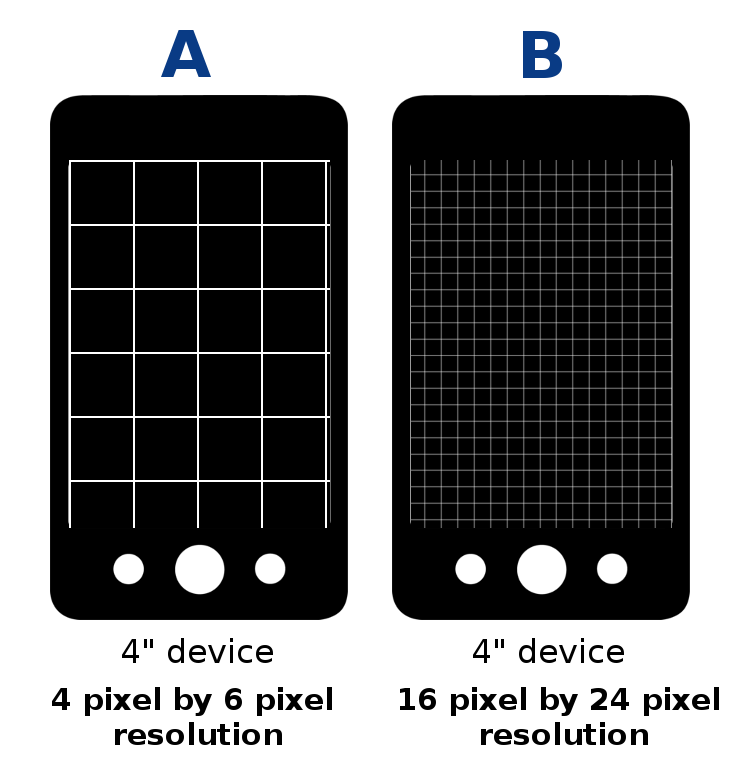
\includegraphics[scale=1]{chapters/ch06/images/2}
\end{center} 

So there are a lot more pixels on device \texttt{B} as compared to device \texttt{A}. Therefore device \texttt{B} is capable of showing much more details and super sharp images as opposed to device \texttt{A}. \textit{As a result, A 3 px by 3 px image on device \texttt{A} will almost fill the screen, but it will look like a tiny dot on device \texttt{B}.} 

As you might have already guessed that it is extremely difficult to make an app that looks almost the same on all devices. For example if we set the size of the widgets in terms of pixels or even physical dimensions such as inches or millimeters, our layout is going to look dramatically different across all devices. A huge problem !

To solve this issue, android OS developers came up with the concept of generic units or ``\textit{Device Independent Pixel}'' units, ``\texttt{dp}'' or ``\texttt{dip}'' for short. When you specify the size of the widgets in your layouts in terms of device independent pixels then android OS will automatically calculate correct pixel size so that the layout looks almost identical on all devices. Remember that everything boils down to pixels at the end!

\begin{quote}
	\textit{Pixel density tells you how many pixels are stuffed in a 1 inch row. This is also known as ``Dots per Inch'' or ``\textbf{dpi}''.}
\end{quote}

In android, 160 dp\textbf{i} (known as medium dots per inch or \texttt{mdpi}) is considered as a reference point. 1 \texttt{dp} is exactly 1 pixel on a (160 dpi) \texttt{mdpi} device. So a button having a width of 50 \texttt{dp} will boil down to 50 pixels wide on a \texttt{mdpi} device. 
Suppose that we have another device having almost same physical screen size as the first device but having 320 \texttt{dpi}. So in this case there are twice as many pixels packed in the same area. Now if our button is to look having consistent size on this device also, it needs to be resized. New size of the button will become $320\div160\times10 = 20$ pixels. So in this case the android OS will \textit{automatically} convert 10 \texttt{dp} to 20 pixels wide button. \\

\textit{Note:} Do not confuse \texttt{dp}/\texttt{dip} with \texttt{dpi}. \texttt{dp} means ``device independent pixels (units)'' whereas \texttt{dpi} stands for ``dots per inch''. These are two completely different things.\\

\subsection{Setting Units Through Design View}
\subsubsection{Create New Project}
\label{ITS:createProj}
Create a new project from scratch. Perform the following steps:
\begin{enumerate}
	\item Create a new project having name ``\texttt{Lec07}''
	\item Select minimum API 16 : Android 4.1 (Jelly Bean).
	\item Select ``\texttt{Empty Activity}''
	\item Accept default values for activity and click finish. \\
\end{enumerate}

\subsection{Setting Units Through Design XML}
\label{ITS:unitXML}
Open up ``\texttt{activity\_main.xml}'' and go to the design mode. Select ``text view'' and change its background color to anything you like. Set it's \texttt{id} to ``\texttt{idText}''. Also set the \texttt{layout:width} to 230 \texttt{px} \textit{(pixels)}. Now cycle through different devices from largest to the smallest and see how \textit{dramatically different} the size of our text view looks on various screens:
\begin{center}
	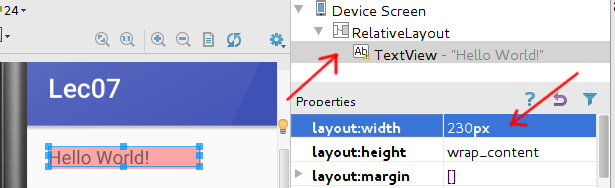
\includegraphics[scale=0.4]{chapters/ch06/images/3}
\end{center} 

After you've performed the task above, change \texttt{layout:width} of the text view to 230 \texttt{\textbf{dp}}. Again cycle through different mobile phones (not the tablets) and observe that this time the size of the text view remains roughly same across all the devices. Tables are special cases because they have a very big physical screen size and a relatively low \texttt{dpi}.

\subsection{Setting Units Through Java Code}
\label{ITS:unitJavaCode}
To make our lives as programmers easier the developers at android have devised different density ``buckets'' within which a device can fall, as shown in table \ref{lec07:densityChart}. Note the third column ``Density factor''. This shows how many more times dense the device is as compared to the standard \texttt{mdpi}. \\

\begin{table}
	\begin{center}
		\begin{tabular}{|l|c|c|}
			\hline \textbf{Generalized density}	& \textbf{dpi} & \textbf{Density factor} \\
			\hline
			\hline \texttt{ldpi} \textit{(low)} & ~120 dpi & \texttt{0.75x} \\
			\hline \texttt{mdpi} \textit{(medium)} &  ~160 dpi & \texttt{1x} \\
			\hline \texttt{hdpi} \textit{(high)} & ~240 dpi & \texttt{1.5x} \\
			\hline \texttt{xhdpi} \textit{(extra-high)} & ~320 dpi & \texttt{2x} \\
			\hline \texttt{xxhdpi} \textit{(extra-extra-high)} & ~480 dpi & \texttt{3x} \\
			\hline \texttt{xxxhdpi} \textit{(extra-extra-extra-high)} & ~640 dpi & \texttt{4x} \\
			\hline 
		\end{tabular} 
	\end{center}
	\caption{Mobile device density table}\label{ITS:densityChart}
\end{table}

Open up \texttt{MainActivity.java}. Inside the \texttt{onCreate} method add the following lines (14, 15):

\begin{center}
	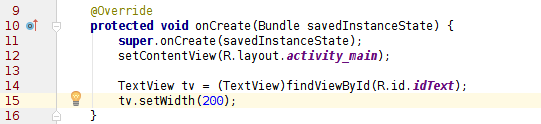
\includegraphics[scale=0.4]{chapters/ch06/images/4}
\end{center} 

\begin{itemize}
	\item Line 14: Get reference of the text view.
	\item Line 15: Set the width of text view. Please note that the \texttt{setWidth} method assumes width in physical ``pixels''.
\end{itemize}

As we've seen in the section \ref{lec07:dp} above that using physical pixels when specifying size is not a good idea. We need to use generalized units but the code only accepts pixels. We are in trouble!

It appears that there is a way to set generalized units through code. First you need to manually get the device density factor and then convert \texttt{dp} units to pixels. Modified code is shown below:

\begin{center}
	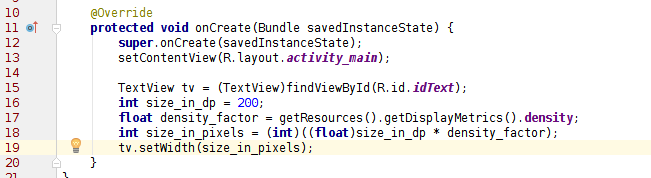
\includegraphics[scale=0.4]{chapters/ch06/images/5}
\end{center} 

Line 17 is an important one. It is getting the density factor of the current device. Then in line 18 we are calculating actual pixels required for the width so that our view looks the correct size on this screen. Since this is Java code, you need to run the app on an emulator or a device to view the changes. More information about ``Display Metrics'' can be found \href{https://developer.android.com/reference/android/util/DisplayMetrics.html}{here}.\\
\\

For more information on supporting multiple screen resolutions and sizes, visit \href{https://developer.android.com/guide/practices/screens_support.html}{here}. Apart from that, \href{https://www.youtube.com/watch?v=zhszwkcay2A}{this video} may prove to be helpful.

You can view device metrics of a lot of devices on \href{https://design.google.com/devices/}{this website}.

\subsection{Exercise}
Create a layout similar to the following. Be sure to set the width of each text view as shown:

\begin{center}
	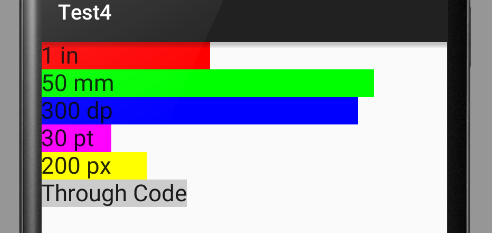
\includegraphics[scale=0.4]{chapters/ch06/images/6}
\end{center} 

Now cycle through the devices. Specially note the size of the blue bar (300 dp). Notice how it re-adjusts itself, looking almost identical on almost all the devices (except for the tablets, as explained in section \ref{lec07:unitXML}).

\section{Displaying Images}
\label{ITS:displayImages}
Table \ref{ITS:densityChart} above shows density chart for different screens. Also from section \ref{ITS:dp} we know that layout sizes should be specified in device independent pixels or \texttt{dp}. Let's see what happens when we try to display a picture on the screen.\\

Following section \ref{lec07:createProj} create a new project and name it \texttt{Lec07b}. Open up \texttt{activity\_main.xml}. Change the text of the default text view to anything such as ``Picture Demo''. \\

Now from devices select 2.7'' QVGA (240x320 : \texttt{ldpi}):

\begin{center}
	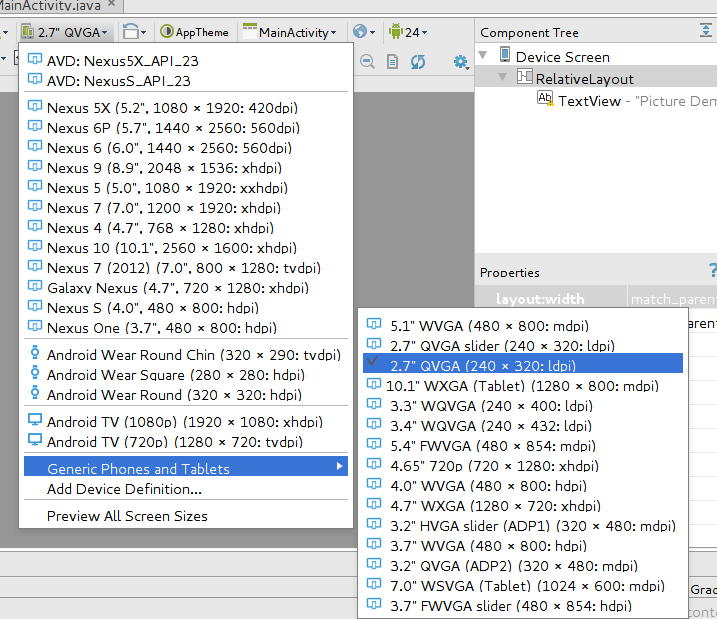
\includegraphics[scale=0.4]{chapters/ch06/images/7}
\end{center}

Unzip \texttt{lec07\_package1.zip} to extract a single png file. Switch to ``Project'' mode so that you can see the actual physical directory structure of the project. Create a new physical folder (not a group) called \texttt{drawable-ldpi} in the \texttt{res} folder and copy the \texttt{150x150} \texttt{smiley\_face.png} file in it:

\begin{center}
	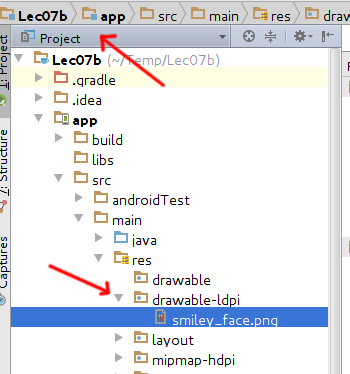
\includegraphics[scale=0.4]{chapters/ch06/images/8}
\end{center}

Now create an image view on the layout and set its source ``\texttt{src}'' to our smiley face i.e \texttt{@drawable/smiley\_face}:

\begin{center}
	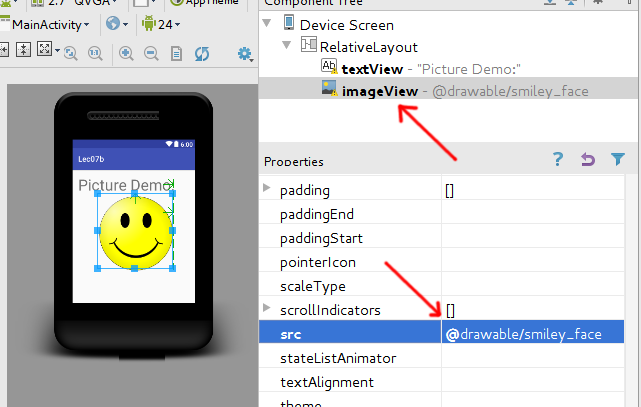
\includegraphics[scale=0.4]{chapters/ch06/images/9}
\end{center}

The \texttt{@drawable} in \texttt{@drawable/smiley\_face} means that it is a picture resource. \texttt{smiley\_face} is the name of the picture file without the file extension. \\

Now select some high \texttt{dpi} device such as Nexus 6. Since we gave the size of picture view in terms of generic units or \texttt{dp}, you can see the android
automatically re-scales everything to match the new resolution (by internally multiplying
everything by density factor). But now uf you zoom in you can see the low resolution picture is being scaled, resulting in a very bad quality pixelated output:

\begin{center}
	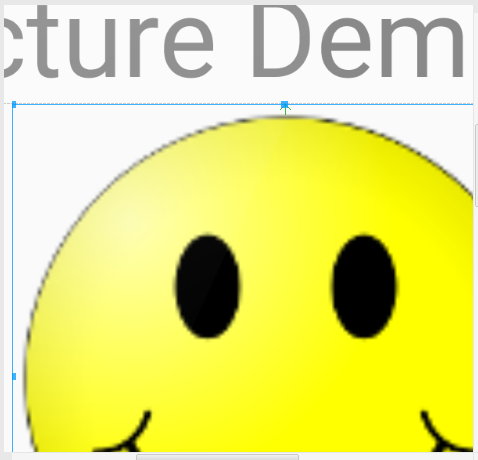
\includegraphics[scale=0.6]{chapters/ch06/images/10}
\end{center}

Fortunately, this is easy to fix. Just make appropriate folders for each \texttt{dpi} and put different size files in them. \textit{\textbf{Very Important:} Even though the sizes are different but the file name should Exactly be the same i.e: ``\texttt{smiley\_face.png}''}. (Unzip \texttt{lec07\_package2.zip} file to get the resources):

\begin{center}
	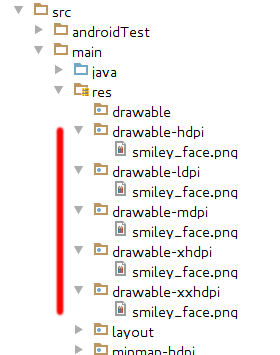
\includegraphics[scale=0.4]{chapters/ch06/images/11}
\end{center}

Refresh the layout view. You should see a super sharp and very crisp image (which the android automatically loads depending upon the pixel density of the device):

\begin{center}
	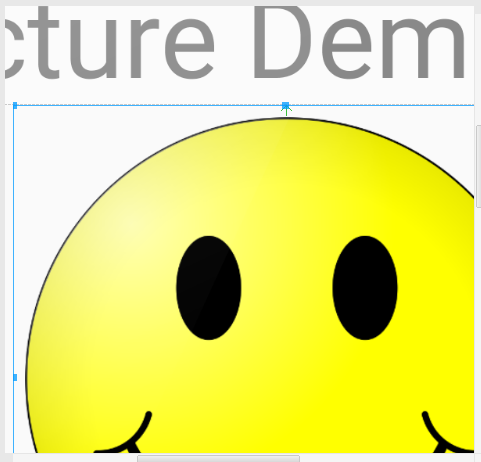
\includegraphics[scale=0.6]{chapters/ch06/images/12}
\end{center}

\vskip 5mm
\textit{\textbf{To summerize:}} In order to maintain highest quality across multiple devices, you must provide multiple sizes for the same picture. Android will automatically choose the correct one depending on the device. 

You design reference or base picture on a \texttt{mdpi} \texttt{1x} density device. Based on that you generate artwork for other densities. For example, if you've created a $100px \times 100px$ artwork for \texttt{mdpi}, according to table \ref{lec07:densityChart} given on page \pageref{lec07:densityChart} you need to create a $200px \times 200px$ graphic for a \texttt{xhdpi} device and a $400px \times 400px$ graphics for \texttt{xxxhdpi} device and so on.

\subsection{Manipulating Images through Code}
Create a new project and open up \texttt{MainActivity.java}. 

\subsection{Exercise}
\begin{enumerate}
	\item Create a new project.
	\item Download the following image:
	
	\url{http://techtalks.ideacellular.com/wp-content/uploads/2015/09/android.jpg}
	
	\item Scale it down to $100px \times 100px$ pixels (use GIMP or MS paint or any of your favorite picture editing software). This image will be used on \texttt{mdpi} as a reference.
	
	\item Select any \texttt{mdpi} device and create an image view on the layout using this image.
	
	\item Now you have to make various sizes of this image by scaling the original hi-res image given in the link above. (again use MS paint). When done, put them in proper folders as described in section \ref{lec07:displayImages}.
	
	\item When you're finished, cycle through various devices. Make sure that the images are properly being selected and displayed depending on the device currently selected.	
\end{enumerate}

\vskip 5mm
For more information about different screen densities visit \href{https://developer.android.com/training/basics/supporting-devices/screens.html}{here} and \href{https://developer.android.com/training/multiscreen/screendensities.html}{here}.


\section{Custom Application Icons}
Sometimes it is much more interesting to specify a custom app launcher icon instead of a green android robot. As we discussed above that there are a huge number of different devices out there. Like pictures we must generate icons having multiple resolutions and put them in proper folders. The folder in which launcher icon resides is known as ``\texttt{mipmap}'':

\begin{center}
	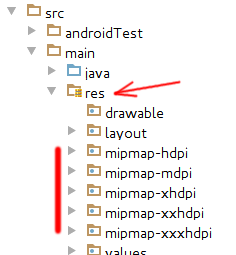
\includegraphics[scale=0.4]{chapters/ch06/images/22}
\end{center}

There are two ways to change the icon, automatically through android studio and manually. 

\subsection{Changing Launcher Icon through Android Studio}
\label{ITS:changingLauncherIconThroughAndroidStudio}
From the project panel, right click on the \texttt{res} folder and select ``New $\rightarrow$ Image Asset''. A dialog box will appear. You can generate a wide variety of icons for many different purposes, but we are interested in launcher icons only:

\begin{center}
	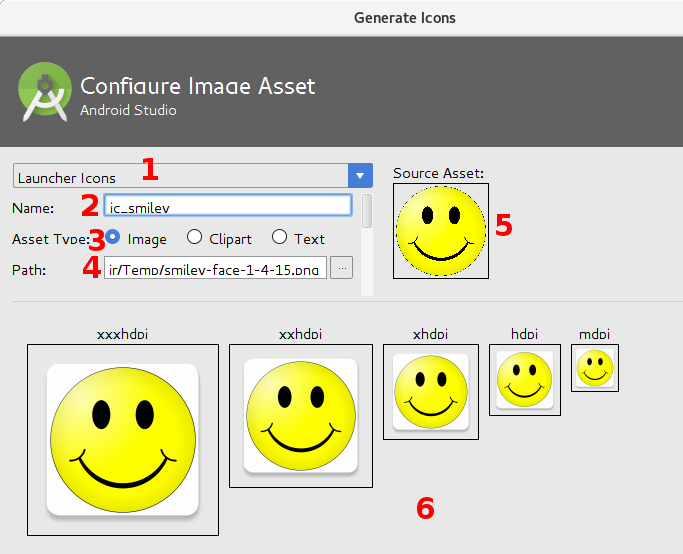
\includegraphics[scale=0.4]{chapters/ch06/images/23}
\end{center}

\begin{enumerate}
	\item Select ``Launcher Icons'' from the combo box because that's what we want to generate.
	\item You can give it any file name you like. Here we give it ``\texttt{ic\_smiley}''
	\item This tells which source will be used to generate the icons. We will be generating icons from our custom image, so select the ``image'' radio button. You can also choose a graphic from the clipart library. Third option is to use plain text to create the icons.
	\item Complete path to our source graphic file. Here we are re-using the smiley graphic from section \ref{lec07:displayImages}.
	\item Preview of the source image.
	\item Preview of the final icons generated for multiple screen densities.
\end{enumerate}

Click next. That will take you to the ``Custom Icon Path'' dialog. Just keep everything as default and hit ``Finish''. Now go to the project panel and look under all these \texttt{mipmap-*} folders. Android studio has automatically generated smiley icon files:

\begin{center}
	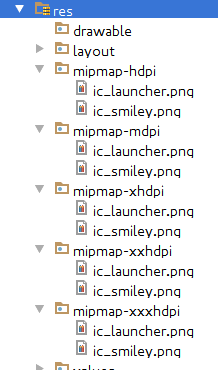
\includegraphics[scale=0.4]{chapters/ch06/images/24}
\end{center}

Now we've got two launcher icons. One final thing is to actually set our new icon in the manifest file. Open up ``\texttt{AndroidManifest.xml}'' file and change the value of the \texttt{android:icon} attribute to ``\texttt{@mipmap/ic\_smiley}'' (line 7):

\begin{center}
	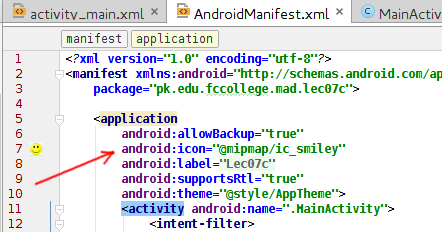
\includegraphics[scale=0.4]{chapters/ch06/images/25}
\end{center}

Build your app and install it on the device. It will now have the brand new smiley icon:

\begin{center}
	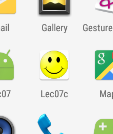
\includegraphics[scale=0.4]{chapters/ch06/images/26}
\end{center}

\subsection{Changing Launcher Icon Manually}
Sometimes we need to change the launcher icons manually because the built-in android studio icon generator is very limited and has got little features. Therefore professional graphic artists may create highly custom icons for your app. You can also generate multiple resolution icons yourself using software such as photoshop or GIMP.

There are other online tools that you can use to easily create launcher icons and give varied special effects to them, including transparency. One such tool is called the ``Android Asset Atudio'' and can be accessed through here:

\url{https://romannurik.github.io/AndroidAssetStudio/}

Following chart shows the exact size of icon you need to generate for a particular density:

\begin{center}
	\begin{tabular}{|c|c|}
		\hline \textbf{Density}	& \textbf{Launcher Icon Size} \\
		\hline
		\hline \texttt{ldpi} & 36 $\times$ 36 px \\
		\hline \texttt{mdpi} & 48 $\times$ 48 px \\
		\hline \texttt{hdpi} & 72 $\times$ 72 px \\
		\hline \texttt{xhdpi} & 96 $\times$ 96 px \\
		\hline \texttt{xxhdpi} & 144 $\times$ 144 px \\
		\hline \texttt{xxxhdpi} & 192 $\times$ 192 px \\
		\hline 
	\end{tabular} 
\end{center}

After generating icon files, you need to place then in appropriate ``\texttt{mipmap-*}'' folder and set the icon from \texttt{AndroidManifest.xml} file. \\

You can view more about launcher icons \href{https://developer.android.com/guide/practices/ui_guidelines/icon_design_launcher.html}{here.}

\subsection{Exercise}
Use the \href{https://romannurik.github.io/AndroidAssetStudio/}{``Android Asset Studio''} to create launcher icons having transparent background. Apply the icons to your app and see how it looks (you can use any graphic file you wish for the source, you can create your own or just search google).

\section{More on Layout Inflater}
\label{ITS:moreOnInflater}
Layout inflater parses a layout xml file and creates java objects from that. We have discussed the layout inflater many times before, such as in Lecture 4 section 3.2. In this section we will actually try to inflate a custom layout xml into a root \texttt{ViewGroup} object through java code. \\

Create a new project from scratch as shown in section \ref{ITS:createProj} and name it anything you like.

Let's first create the XML layout file. In the project panel, under the \texttt{res} folder/group, right click on \texttt{layout} folder and select ``New $\rightarrow$ Layout Resource File''. You can give the new layout file any name you like but for this tutorial we will call it ``\texttt{my\_layout}''. A new layout xml file will be created inside the \texttt{layout} folder:

\begin{center}
	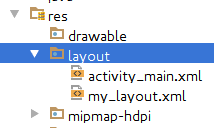
\includegraphics[scale=0.4]{chapters/ch06/images/30}
\end{center}

Open up \texttt{my\_layout.xml} and use your imagination to create a reasonable fun layout. I came up with the following (two text views and one image view all inside a root layout):

\begin{center}
	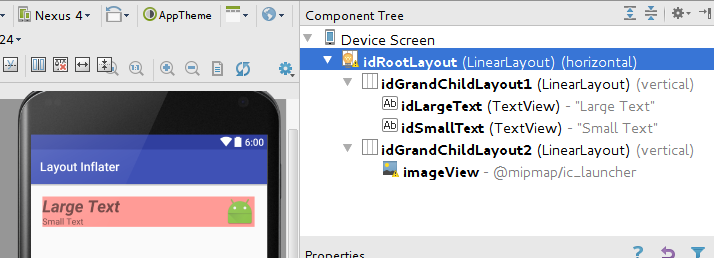
\includegraphics[scale=0.4]{chapters/ch06/images/31}
\end{center}

\textbf{\textit{Important:}} You MUST specify a root layout which contains everything else (like \texttt{idRootLayout} is the root that contains everything else in the above example). \\

Alright, we've just made our custom layout that we will be inflating inside a \texttt{ViewGroup} through java code. Open up \texttt{activity\_main.xml} and make a layout similar to the following, observing the component tree at the right side (assign the \texttt{id}s as shown):

\begin{center}
	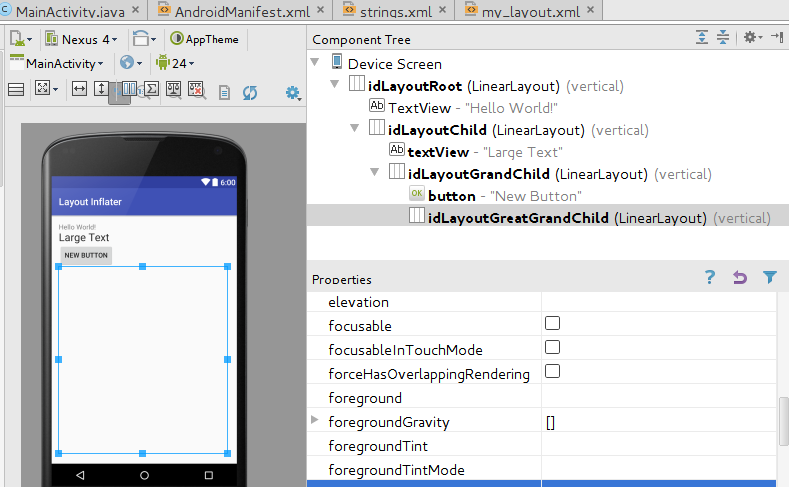
\includegraphics[scale=0.4]{chapters/ch06/images/32}
\end{center}

If you run the app on a device you will see the following:

\begin{center}
	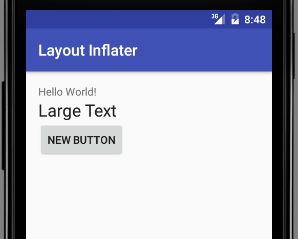
\includegraphics[scale=0.4]{chapters/ch06/images/33}
\end{center}


We will be inflating our custom layout inside the great grand child linear layout having the id \texttt{idLayoutGreatGrandChild}. Open up \texttt{MainActivity.java} and inside the \texttt{onCreate} method add the following code (lines 16 to 18):

\begin{center}
	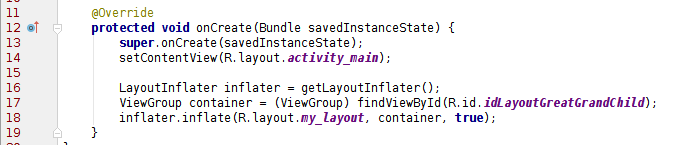
\includegraphics[scale=0.4]{chapters/ch06/images/34}
\end{center}

Let's analyze the code line by line:
\begin{itemize}
	\item \textit{Line 16:} Save the reference to the global inflater object using \texttt{getLayoutInflater()} method.
	
	\item \textit{Line 17:} Here we are getting the reference to the \texttt{ViewGroup} in which we want to inflate our custom layout.
	
	\item \textit{Line 18:} This line is important! The \texttt{inflate} method does all the heavy lifting of inflating the layout xml into a view group. It takes three parameters.
	\begin{itemize}
		\item \textit{$1^{st}$ Parameter: } The \texttt{id} of the layout that you want to inflate
		
		\item \textit{$2^{nd}$ Parameter: } This is the view group container object within which the layout will be inflated to.
		
		\item \textit{$3^{rd}$ Parameter: } By default this is set to \texttt{true}. If this is \texttt{true} then the layout will be inflated inside and attached to the root view group container given in the second parameter. 
		
		\textit{But if this parameter is \texttt{false} then the inflated layout will NOT attach itself or inflate into the root container given in the second parameter}. Instead the inflater will return a new view group object containing the inflated layout. But you STILL need to give the root in the $2^nd$ parameter for correct output. 
		
		Google's documentation is really \textit{Vague} on this !!!
	\end{itemize}
\end{itemize}

Since the third parameter of the \texttt{inflater} method was set to \texttt{true}, the layout was inflated in the view group great grand child given in the second parameter. If you run the app, you will see our custom layout inside the view group we chose:

\begin{center}
	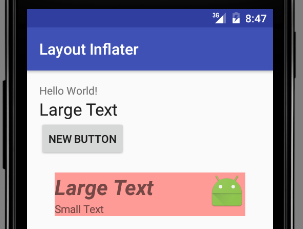
\includegraphics[scale=0.4]{chapters/ch06/images/35}
\end{center}

Now let's set the third parameter of the \texttt{inflater} metod to \texttt{false}. Modify the code as follows:

\begin{center}
	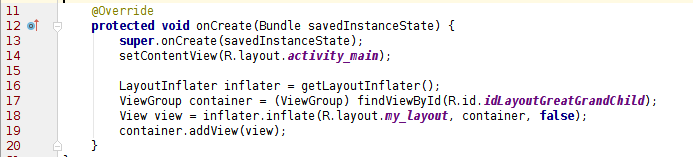
\includegraphics[scale=0.4]{chapters/ch06/images/36}
\end{center}

In this case the \texttt{inflater} method is returning a \texttt{View} object containing our custom inflated layout. Then you can add this view object to any \texttt{ViewGroup} using the \texttt{addView} method (line 19 in the above code).

If you run this code, you will see exactly the same output as before. Two ways to do the same thing! \\

For more information on layout inflater visit \href{https://www.bignerdranch.com/blog/understanding-androids-layoutinflater-inflate/}{here},  \href{https://developer.android.com/reference/android/view/LayoutInflater.html}{here} and \href{https://developer.android.com/reference/android/view/LayoutInflater.html#inflate(int,%20android.view.ViewGroup,%20boolean)}{here}.
	
	\section{Toasts}
	Create a new project from scratch as shown in section \ref{lec07:createProj} and name it anything you like.
	
\subsection{Toast Basics}
\label{lec07:toastBasics}
\begin{quote}
	\textit{``\texttt{Toast} is just a short message that appears on the screen for a small amount of time.''}
\end{quote}

To get a better idea, let's create a Toast. Open up \texttt{MainActivity.java} and inside the \texttt{onCreate} method, type the following code (lines 15 to 20):

\begin{center}
	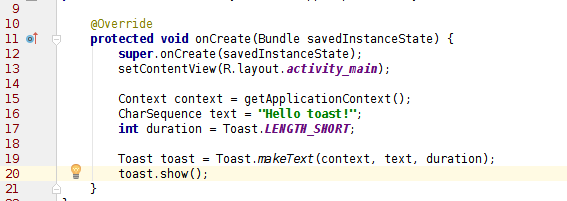
\includegraphics[scale=0.4]{chapters/ch06/images/13}
\end{center}

The way to create a toast is to call the static method provided in the \href{https://developer.android.com/reference/android/widget/Toast.html}{\texttt{Toast}} class named \texttt{makeText}. There are multiple overloaded \texttt{makeText} methods but the one we are interested in takes three arguments. First one is the context, second is the actual text to display and the third is the length of time this toast will be displayed. 

Once the toast object is created, you need to explicitly call the \texttt{show} method which does the job of actually displaying it on the screen.

\begin{quote}
	``\textit{\textbf{Tip:}} Most common mistake while troubleshooting \texttt{Toast} related issues is to forget to call the \texttt{show} method at the end.''
\end{quote}

Let's analyze the above code in detail:
\begin{itemize}
	\item \textit{Line 15:} Get the application context. You can think of the \href{https://developer.android.com/reference/android/content/Context.html}{\texttt{Context}} as a global reference to the entire app. This object contains system level settings that maybe required by the toast object. Instead of a global application context we can also pass here ``\texttt{this}'' or ``\texttt{MainActivity.this}'' or ``\texttt{\textit{AnyActivity}.this}''.
	
	\item \textit{Line 16:} This is the text message that we want to display on the screen.
	
	\item \textit{Line 17:} The amount of time this toast will be displayed on to the screen. Currently there are two default values \texttt{Toast.LENGTH\_SHORT} which is defined to be $0$ and \texttt{Toast.LENGTH\_LONG} which is defined to be a constant $1$.
	
	\item \textit{Line 19:} Here we are creating the toast using \texttt{makeText} static method and then passing all the necessary arguments.
	
	\item \textit{Line 20:} Finally we call the \texttt{show} method to display he toast on the screen.
\end{itemize}

When you run the app following toast appears for a short duration near the bottom edge of the device:

\begin{center}
	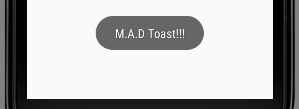
\includegraphics[scale=0.4]{chapters/ch06/images/14}
\end{center}

You can also combine the code in above listing in a single line as follows (line 15). We are NO longer creating the toast object ``\textit{explicitly}'':

\begin{center}
	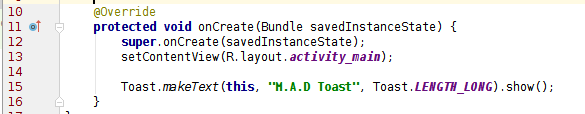
\includegraphics[scale=0.4]{chapters/ch06/images/15}
\end{center}


\subsection{Toast Position}
What if we want the toast to display at the top of the screen instead of the default bottom. We can use the ``\texttt{setGravity}'' method on the toast object as shown in line 17 below:

\begin{center}
	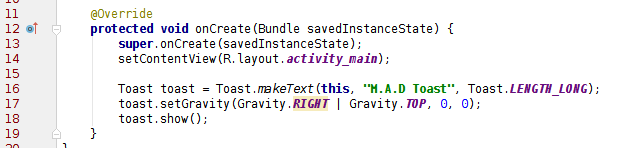
\includegraphics[scale=0.4]{chapters/ch06/images/16}
\end{center}

We can combine different gravity options using the pipe ``\texttt{|}'' operator. Run the app and the toast will be displayed in the upper right corner of the app:

\begin{center}
	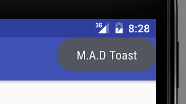
\includegraphics[scale=0.4]{chapters/ch06/images/17}
\end{center}

\underline{\textbf{Pop Quiz:}} What do the remaining two parameters in the ``\texttt{setGravity}'' do? Currently both of them are set to 0. Try changing these and see how the toast behaves.

\subsection{Custom Toasts}
You can even change the outlook of the toast message. For that we first need to create a (fairly complex) layout having a \texttt{ViewGroup} at the \texttt{root} position. Then we need to \texttt{inflate} (Lec05, section 3.2) the xml layout into java view object. Finally we need to set this view as the toast's new outlook. \\

As we did in section \ref{lec07:moreOnInflater}, create a layout file and call it ``\texttt{my\_toast\_layout}''.

Open up ``\texttt{my\_toast\_layout.xml}'' and try to create a layout roughly matching the following figure. The hierarchical structure and the \texttt{id}'s of all the components are shown in the component tree to the right:

\begin{center}
	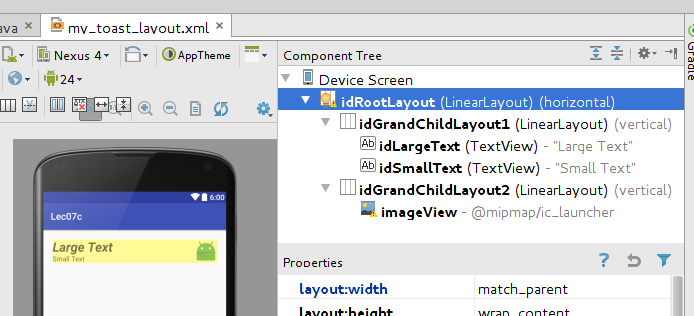
\includegraphics[scale=0.4]{chapters/ch06/images/19}
\end{center}

Now open up \texttt{MainActivity.java} and modify the \texttt{onCreate} method as follows (lines 20 to 34):

\begin{center}
	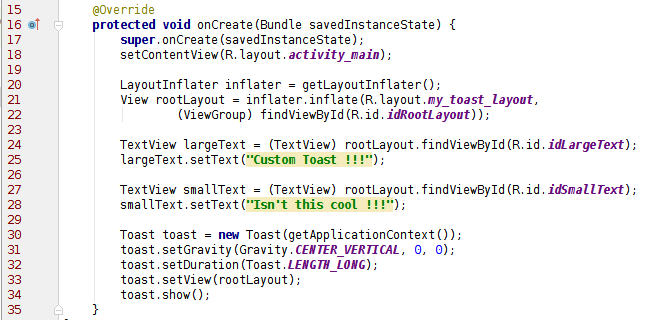
\includegraphics[scale=0.4]{chapters/ch06/images/20}
\end{center}

\begin{itemize}
	\item \textit{Line 20:} Get the \href{https://developer.android.com/reference/android/view/LayoutInflater.html}{\texttt{LayoutInflater}} object.
	
	\item \textit{Line 21-22:} Calls the \texttt{inflate} method on the inflater object. The \texttt{inflate} method takes two parameters, the first one is the layout XML resource id which will be inflated, the second is the \texttt{id} of the root element.
	
	\item \textit{Line 24-28:} Since we've now got the reference to the root element in ``\texttt{rootLayout}'' variable, we are now simply finding the text views and setting their texts.
	
	\item \textit{Line 30-32:} These should already be familiar to you. We've seen these in the section \ref{lec07:toastBasics}.
	
	\item \textit{Line 33:} The \texttt{setView} method is taking the inflated object as a parameter and attaching it to the toast object.
	
	\item \textit{Line 34:} Finally we call the \texttt{show} method to display the toast on the screen.
	
\end{itemize}

When you run the app, you will see a toast bearing our custom layout being displayed in the center of the screen:

\begin{center}
	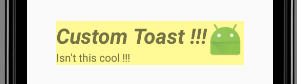
\includegraphics[scale=0.4]{chapters/ch06/images/21}
\end{center}

More information about \texttt{Toasts} can be viewed \href{https://developer.android.com/guide/topics/ui/notifiers/toasts.html}{here}.

\section{Playing Sound}

